\documentclass[a4paper,10pt]{article}

\usepackage{amsfonts}
\usepackage{amssymb}
\usepackage{latexsym}
\usepackage{graphicx}
\usepackage{amssymb,amsmath}
\usepackage{listings}
\usepackage[titletoc]{appendix}
\usepackage{courier}

\linespread{1}

\hoffset -1in \topmargin 0mm \voffset 0mm \headheight 0mm
\headsep0mm
\oddsidemargin  20mm     %   Left margin on odd-numbered pages.
\evensidemargin 20mm     %   Left margin on even-numbered pages.
\textwidth   170mm       %   Width of text line.
\textheight  252mm

\makeatletter
\renewcommand\@openbib@code{%
     \advance\leftmargin  \z@ %\bibindent
      \itemindent \z@
     % Move bibitems close together
     \parsep -0.8ex
     }
\makeatother

\makeatletter
\renewcommand\section{\@startsection {section}{1}{\z@}%
                                   {-3.5ex \@plus -1ex \@minus -.2ex}%
                                   {2.3ex \@plus.2ex}%
                                   {\large\bfseries}}
\makeatother

\makeatletter
\renewcommand\subsection{\@startsection {subsection}{1}{\z@}%
                                   {-3.5ex \@plus -1ex \@minus -.2ex}%
                                   {2.3ex \@plus.2ex}%
                                   {\normalsize\bfseries}}
\makeatother

\begin{document}
\pagestyle{empty}

\begin{center}
{\bf \Large UNBIASED ESTIMATION OF PERMUTATION ENTROPY IN ALZHEIMER'S DISEASE DIAGNOSIS FROM EEG}
\end{center}

\smallskip
\begin{center}
{\large V\'{a}clav Hubata--Vacek $^1$, Jarom\'{i}r Kukal $^1$, Lucie Tylov\'{a} $^1$, Old\v{r}ich Vy\v{s}ata $^{2,3}$}
\end{center}

\smallskip
\begin{center}
$^1$CTU in Prague, Faculty of Nuclear Sciences and Physical Engineering\\
Department of Software Engineering in Economics\\
B\v{r}ehov\'{a} 7, 115 19 Prague 1 \\
Czech Republic\\
hubatvac@fjfi.cvut.cz\\
 ~\\
$^2$ICT in Prague, Faculty of Chemical Engineering\\
Department of Computers and Control Engineering\\
Technick\'{a} 5, 160 00 Prague 6 \\
Czech Republic\\
 ~\\
$^3$Charles University in Prague , Faculty of Medicine in Hradec Kralove\\
Department of Neurology\\
Simkova 870, 500 38 Hradec Kralove 1 \\
Czech Republic\\
 ~\\

\end{center}

\bigskip
\noindent Abstract: \textit{EEG signal of healthy patient can be recognized as output of a chaotic system. There are many measures of chaotic behavior: Hurst and Lyapunov exponents, various dimensions of attractor, various entropy measures, etc. We prefer permutation entropy of equidistantly sampled data. The novelty of our approach is in bias reduction of permutation entropy estimates, memory decrease, and time complexities of permutation analysis. Therefore, we are not limited by EEG signal and permutation sample lengths. This general method was used for channel by channel analysis of Alzheimer diseased (AD) and healthy (CN) patients to point out the differences between AD and CN groups.}

\vspace*{10pt} \noindent Keywords: \textit{EEG, Alzheimer's disease, permutation entropy, unbiased estimation, hash table}


\bigskip
\section {Introduction }
Alzheimer�s disease (AD) is the most common form of dementia, which gradually destroys the host�s brain cells. Recent findings estimate that 35 million people worldwide currently suffer from AD. Clinically, AD manifests itself as a slowly progressing impairment of mental functions whose course lasts several years prior to the death of the patient. Structural changes in AD are related to the accumulation of amyloid plaques between nerve cells in the brain and with the appearance of neurofibrillary tangles inside nerve cells, particularly in the hippocampus and the cerebral cortex. Although a definite diagnosis is possible only by necropsy, a differential diagnosis with other types of dementia and with major depression should be attempted. Magnetic resonance imaging and computerized tomography can be normal in the early stages of AD, but a diffuse cortical atrophy is the main sign in brain scans. Mental status tests are also useful. Electroencephalography (EEG)  is a non-invasive technique that was first used by Hans Berger in 1929 to record electrical activity of the human brain. The EEG has been used as a tool for investigating dementias for several decades. The conventional spectral analysis of EEG has mainly been concerned with spectral features in several frequency bands. Although the spectral analysis has been successful in AD studies, nonlinear dynamic analysis is crucial if trying to capture higher order dynamic properties of the brain. In particular, several authors have analyzed the EEG in AD patients with non-linear methods. It has been shown that AD patients have lower correlation dimension ($D_{2}$) values as a measure of the underlying system dimensional complexity � than control subjects [\ref{bib11}]. Furthermore, AD patients also have significantly lower values of the largest Lyapunov ($\lambda_{1}$) exponent than controls in almost all EEG channels. However, estimating the non-linear dynamic complexity of physiological data using measures such as $D_{2}$ and $\lambda_{1}$ is problematic, as the amount of data required for meaningful results in their computation is beyond the experimental possibilities for physiological data [\ref{bib12}]. One alternative solution lies in computing the entropy of the EEG [\ref{bib8}]. The concept of entropy has achieved a large consensus as an indicator of complexity of nonlinear signals [\ref{bib7}], [\ref{bib13}]. A number of variants of this notion have been proposed in the literature which show different degrees of flexibility, relevance to different problems, efficiency in their computation, as well as theoretical foundations. This work investigates the potential of complexity analysis of multidimensional EEG as indicator of AD onset through permutation entropic modeling.

\section {Permutation entropy }

\subsection {Shanon entropy and its estimation}
\textbf{Definition.} Shannon entropy [\ref{bib5}] $ H_{\mbox{\scriptsize{S}}} $ of a discrete random variable $X$ with possible values $x_{1}, ..., x_{m}$ and probability mass function $p(X)$ is defined as
\begin{equation}
\label{eq:shannonentro}
H_{\mbox{\scriptsize{S}}}=-\sum_{i=1}^{m} p_{i} \ln{p_{i}},
\end{equation} 
where $p_{i}=p(x_{i})$.\\
\\*
If the probability function is unknown for an experimental data set, and the number of possible values is finite for random variable $X$, we estimate probalility function $p_{i}$ by relative frequency $p_{j,\mbox{\scriptsize{N}}}$ and number of events $k_{\mbox{\scriptsize{N}}}$ as
\begin{equation}
\label{eq:pjn}
p_{j,\mbox{\scriptsize{N}}} = \frac{n_{j}}{n},
\end{equation} 
\begin{equation}
\label{eq:k}
k_{\mbox{\scriptsize{N}}} = \sum_{n_{j}>0}{1} \leq k, 
\end{equation} 
where $n_{j}$ is the number of occurrences $x_{i}$ of random variable $X$, and $n$ the total number of measurement results. Then we get \textit{naive estimate} of Shannon entropy as
\begin{equation}
\label{eq:seestimate}
H_{\mbox{\scriptsize{N}}}=-\sum_{j=1}^{k_{\mbox{\scriptsize{N}}}} p_{j,\mbox{\scriptsize{N}}} \ln{p_{j,\mbox{\scriptsize{N}}}}.
\end{equation} 
This estimate is biased, and therefore it has a systematic error. \\
\\*
Miller [\ref{bib2}] modified \textit{naive estimate} $H_{\mbox{\scriptsize{N}}}$ using first order Taylor expansion, which produces better estimation
\begin{equation}
\label{eq:miller}
H_{\mbox{\scriptsize{M}}}=H_{\mbox{\scriptsize{N}}} + \frac{k_{\mbox{\scriptsize{N}}}-1}{2n}.
\end{equation} 

\subsection {Application to permutation analysis }

Entropy estimates can be easily applied to permutation event analysis [\ref{bib3}],[\ref{bib4}]. Methodology from [\ref{bib2}] estimates a smaller bias. Let time series be \{$a_{k}$\}$_{k=1}^{T}$ and sliding window \{$b_{k}$\}$_{k=1}^{w}$ of length $w$, then we can substitute signal values $b_{k}$ in the window with their orders and then obtain permutation pattern \{$\pi_{k}$\}$_{k=1}^{w}$. The process of pattern conversion is depicted in Fig. \ref{img:top}. \\
\\*
The universe of random variable $X$ is a set of all permutation of length $w$. Therefore, the number of possible permutations is
\begin{equation}
\label{eq:mwfac}
m = w!,
\end{equation} 
but the number of various permutations in given signal cannot exceed the number of sliding samples as
\begin{equation}
\label{eq:kn}
k_{n} \leq n = T-w+1.
\end{equation} 
The number of occurences of $j^{\mbox{th}}$ permutation pattern corresponds with $n_{j}$, and $n$ is the total number of samples. Now, we can directly use (\ref{eq:seestimate}) and calculate the biased naive estimation $H_{\mbox{\scriptsize{N}}}$ as in [\ref{bib5}].
Our methodology is based on Miller's approach [\ref{bib2}] and direct application of (\ref{eq:miller}) to permutation patterns.

\section {Permutation analysis for large samples }

The main disadvantage of the original procedure of permutation analysis [\ref{bib3}] is in its memory and time complexities. They realized permutation memory as a matrix of $w$ columns and $w$! rows together with counter vector of length $w$!. It enables permutation analysis only for $w < 13$ on a typical computer. The time complexity of single permutation counting is also $w$!, in the worst case. Therefore, we decided to use more sophisticated data structure for permutation analysis.
There are many data structures and algorithms for realizing of \textit{look-up table} as a kind of memory with fast access. Our memory has to be optimized only for two operations: FIND and INSERT. We used \textit{hash table} with open addressing and linear probe strategy [\ref{bib6}] as a model, which is easy to realize.
Let $P > n$ be the optional prime number. Then the \textit{loading factor} is defined as a ratio $\alpha = n/P < 1$. The mean number of permutation vector comparisons during successful FIND operation was determined [\ref{bib6}] as
\begin{equation}
\label{eq:etopt}
\mbox{E}T_{\mbox{\scriptsize{OPT}}} = \frac{1}{2}\left(1+\frac{1}{1-\alpha}\right).
\end{equation}
In the case of unsuccessful FIND operation and INSERT operation, the mean number of permutation vector comparisons is higher [\ref{bib6}] than in the previous optimistic case
\begin{equation}
\label{eq:etpes}
\mbox{E}T_{\mbox{\scriptsize{PES}}} = \frac{1}{2}\left(1+\frac{1}{(1-\alpha)^2}\right).
\end{equation}
Our tiny and fast implementation of  permutation memory is a matrix of occurred permutations with $w$ columns and $P > n$ rows together with counter vector of length $P$. The time complexity of single permutation counting is constant and dependent only on loading factor in the best (\ref{eq:etopt}) and worst (\ref{eq:etpes}) cases. It enables very fast permutation analysis for higher sample length $w$ and long EEG sequences.
The last implementation detail is how to realize hash function $index = \mbox{h}(\boldsymbol{\pi})$ for given permutation pattern $\boldsymbol{\pi}$. By substracting vector of units from vector $\boldsymbol{\pi}$, we obtain digital form $\boldsymbol{y} = \boldsymbol{\pi} - 1$ in the first step. Let $R = w$ be the base of digital system. In the second step, we calculate the value $v$ of $\boldsymbol{y}$ according to base $R$. The resulting index into hash table has a value $index = v \bmod P$. In the case of Matlab environment, we must increase the index by one.
In the case when $P > 3n$, we have $\alpha < 1/3$ and then the mean number of trials is less than 1.25 in the optimistic case (\ref{eq:etopt}) and less than 1.625 in the pessimistic (\ref{eq:etpes}). The source Matlab code for single time series analysis is included in the Appendix.

\section {Application to EEG }

Permutation entropy was applied to EEG signals obtained from two groups of patients. The first group is represented by 10 patients with Alzheimer's disease (AD), and the second group is represented by 10 healthy patients (CN). EEG signals for each patient are recorded from 19 electrodes placed on the scalp. Time series length $T$ varies between 70000 and 120000. Using sampling frequency 200 Hz, we tried to separate these two groups of patients by two-sample t-test with null hypotheses and alternative hypothesis as
\begin{equation}
\label{eq:hypothesis0}
\mbox{H}_{0}: \mbox{E}\hat{H}(\mbox{AD})=\mbox{E}\hat{H}(\mbox{CN}),
\end{equation}
\begin{equation}
\label{eq:hypothesis1}
\mbox{H}_{\mbox{A}}: \mbox{E}\hat{H}(\mbox{AD}) \neq \mbox{E}\hat{H}(\mbox{CN}).
\end{equation} 
The final results for permutation entropy estimators $H_{\mbox{\scriptsize{N}}}$ and $H_{\mbox{\scriptsize{M}}}$ are in Tabs. \ref{tab:naiveestimate} and \ref{tab:millerestimate}.\\
\\*
First, we evaluated separation ability of naive estimate $H_{\mbox{\scriptsize{N}}}$ of Shannon etropy $H_{\mbox{\scriptsize{S}}}$. Using False Discovery Rate (FDR) [\ref{bib1}] methodology of multiple testing for 19 channels and $\alpha = 0.05$ together with t-test, we obtained $\alpha_{\mbox{\scriptsize{FDR}}} = 0.0413$ from $p_{\mbox{\scriptsize{value}}}$ in the Tab. \ref{tab:naiveestimate}. The mean values of $H_{\mbox{\scriptsize{N}}}$ in AD group are less than the mean values of $H_{\mbox{\scriptsize{N}}}$ in CN group for all channels. However, the differences are significant only in frontal channels $ch=1..17$ in the sense of FDR.\\
\\*
Then we evaluated separation ability of Miller estimate $H_{\mbox{\scriptsize{M}}}$ of Shannon etropy $H_{\mbox{\scriptsize{S}}}$. Using the same method as above, we obtained $\alpha_{\mbox{\scriptsize{FDR}}} = 0.0216$ from $p_{\mbox{\scriptsize{value}}}$ in Tab. \ref{tab:millerestimate}. Mean values of $H_{\mbox{\scriptsize{M}}}$ in AD group are
still less than mean values of $H_{\mbox{\scriptsize{M}}}$ in CN group for all channels, and the diferences are significant only in frontal channels $ch=1..12,14,17$ in the sense of FDR which is in better agreement with neurological theories. \\
\\*
Top 10 permutations for two typical patients are depicted on Fig. \ref{img:compare}, where permutations for CN group are more chaotic. Results for channel 8 and window 14 are depicted Fig. \ref{img:boxes} in form of box graph.

\section {Conclusion }
Using Miller's approach instead of direct calculation of Shannon's entropy from permutation frequencies, we have developed a novel method of ECG analysis via permutation entropy. The second advantage of our method is in its very fast permutation analysis and low consumption of computer memory which enables analysis of large time series with greater length of permutation patterns. When the method was applied to diagnose Alzheimer�s disease from 19 channel EEG, we recommended pattern length $w = 14$ and Miller estimate of permutation entropy to achieve the best separation between AD and CN groups in standard two-sided two-sampled t-test. 

\vspace*{10pt} \noindent {\bf Acknowledgement:} The paper was created with the support of CTU in Prague, Grant SGS11/165/OHK4/3T/14.

\begin{thebibliography}{99}
\vskip12pt
\bibitem{bib1}\label{bib1} Benjamini Y., Hochberg Y., \textit{Multiple hypotheses testing with weights}. Scandinavian Journal of Statistics, 24 407-418.
\bibitem{bib2}\label{bib2} Miller G., \textit{Note on the bias of information estimates}. Information Theory in Psychology: Problems and Methods, pp. 95-100 (1955).
\bibitem{bib3}\label{bib3} Bandt C., Pompe B., \textit{Permutation Entropy: A Natural Complexity Measure for Time Series}. Physical Review Letterss, 88, 174102 (2002).
\bibitem{bib4}\label{bib4} Cao Y., Tung W., Gao J. B., Protopopescu V. A., Hively L. M., \textit{Detecting dynamical changes in time series using the permutation entropy}. Physical review E 70, 046217 (2004).
\bibitem{bib5}\label{bib5} Shannon C. E., \textit{A mathematical theory of communication}. Bell System Technical Journal (1948)
\bibitem{bib6}\label{bib6} Knuth D. E., \textit{Art of Programming}. Volume 3: Sorting and Searching, Addison-Wesley, Reading (1998).

\bibitem{bib7}\label{bib7} Pincus S. M., \textit{Approximate entropy as a measure of system complexity}. Proc. Nati. Acad. Sci. USA, Vol. 88, pp. 2297-2301 (March 1991).
\bibitem{bib8}\label{bib8} Ab\'{a}solo D., Hornero R., Espino P., \textit{Approximate Entropy of EEG Background Activity in Alzheimer's Disease Patients}. Intelligent Automation and Soft Computing, Vol. 15, No. 4, pp. 591-603 (2009).
\bibitem{bib11}\label{bib11} Tang S., Jiang X., Liu Z., Ma L., Zhang Z., Zheng Z., \textit{Entropy Analysis in Interacting Diffusion Systems on Complex Networks}. International Journal of Mathematics and Computers in Simulation, ISSN: 1998-0159 (2012).
\bibitem{bib12}\label{bib12} Morabito F. C., Labate D., Foresta F. L., Bramanti A., Morabito G., Palamara I., \textit{Multivariate Multi-Scale Permutation Entropy for Complexity Analysis of Alzheimer�s Disease EEG}. ISSN 1099-4300, 14, 1186-1202; doi:10.3390/e14071186 (2012).
\bibitem{bib13}\label{bib13} Jeong-Hyeon Park, Sooyong Kim, Cheol-Hyun Kim, Andrzej Cichocki, Kyungsik Kim, \textit{Multiscale entropy analysis of EEG from patients under different Pathological Conditions}. Fractals, Vol. 15, No. 4 399�404 (2007).

\end{thebibliography}

\begin{table}[p] 
\begin{center}
\caption{Naive estimate of permutation entropy ($ch$ = 5)}
\label{tab:naiveest5ch}
\begin{tabular}{|l|l|l|l|}
\hline
\multicolumn{1}{|c|}{Window} & \multicolumn{2}{c|}{ Mean $ H_{\mbox{\scriptsize{N}}} $ } & \multicolumn{1}{c|}{$p_{\mbox{\scriptsize{value}}}$} \\
\cline{2-3}
 & \multicolumn{1}{|c|}{AD} & \multicolumn{1}{|c|}{CN} & \\
\hline
4 & 2.5386 & 2.5446 & 0.933709 \\ 
5 & 3.6468 & 3.6643 & 0.883681 \\ 
6 & 4.8405 & 4.8817 & 0.809546 \\ 
7 & 6.0974 & 6.1751 & 0.730612 \\ 
8 & 7.3595 & 7.4887 & 0.638650 \\ 
9 & 8.4999 & 8.7202 & 0.466233 \\ 
10 & 9.3965 & 9.7283 & 0.251339 \\ 
11 & 10.0401 & 10.4452 & 0.094385 \\ 
12 & 10.4718 & 10.8906 & 0.023466 \\ 
13 & 10.7439 & 11.1292 & 0.006136 \\ 
\hline
\end{tabular}
\end{center}
\end{table} 

\begin{table}[p] 
\begin{center}
\caption{Miller estimate of permutation entropy ($ch$ = 5)}
\label{tab:milest5ch}
\begin{tabular}{|l|l|l|l|}
\hline
\multicolumn{1}{|c|}{Window} & \multicolumn{2}{c|}{ Mean $ H_{\mbox{\scriptsize{M}}} $ } & \multicolumn{1}{c|}{$p_{\mbox{\scriptsize{value}}}$} \\
\cline{2-3}
 & \multicolumn{1}{|c|}{AD} & \multicolumn{1}{|c|}{CN} & \\
\hline
4 & 2.5388 & 2.5447 & 0.934097 \\ 
5 & 3.6476 & 3.6649 & 0.884850 \\ 
6 & 4.8441 & 4.8846 & 0.813263 \\ 
7 & 6.1129 & 6.1871 & 0.742882 \\ 
8 & 7.4110 & 7.5299 & 0.671068 \\ 
9 & 8.6248 & 8.8262 & 0.524563 \\ 
10 & 9.6144 & 9.9311 & 0.313112 \\ 
11 & 10.3452 & 10.7512 & 0.134122 \\ 
12 & 10.8452 & 11.2802 & 0.037469 \\ 
13 & 11.1666 & 11.5731 & 0.008713 \\ 
\hline
\end{tabular}
\end{center}
\end{table} 

\begin{table}[p] 
\begin{center}
\caption{Naive estimate of permutation entropy ($ch$ = 8)}
\label{tab:naiveest8ch}
\begin{tabular}{|l|l|l|l|}
\hline
\multicolumn{1}{|c|}{Window} & \multicolumn{2}{c|}{ Mean $ H_{\mbox{\scriptsize{N}}} $ } & \multicolumn{1}{c|}{$p_{\mbox{\scriptsize{value}}}$} \\
\cline{2-3}
 & \multicolumn{1}{|c|}{AD} & \multicolumn{1}{|c|}{CN} & \\
\hline
4 & 2.6227 & 2.6763 & 0.289642 \\ 
5 & 3.7898 & 3.8901 & 0.245163 \\ 
6 & 5.0485 & 5.2067 & 0.210272 \\ 
7 & 6.3754 & 6.6048 & 0.178109 \\ 
8 & 7.7024 & 8.0207 & 0.136442 \\ 
9 & 8.8811 & 9.3133 & 0.070555 \\ 
10 & 9.7614 & 10.2749 & 0.022015 \\ 
11 & 10.3455 & 10.8547 & 0.004363 \\ 
12 & 10.6971 & 11.1372 & 0.001093 \\ 
13 & 10.8891 & 11.2568 & 0.001305 \\ 
\hline
\end{tabular}
\end{center}
\end{table} 

\begin{table}[p] 
\begin{center}
\caption{Miller estimate of permutation entropy ($ch$ = 8)}
\label{tab:milest8ch}
\begin{tabular}{|l|l|l|l|}
\hline
\multicolumn{1}{|c|}{Window} & \multicolumn{2}{c|}{ Mean $ H_{\mbox{\scriptsize{M}}} $ } & \multicolumn{1}{c|}{$p_{\mbox{\scriptsize{value}}}$} \\
\cline{2-3}
 & \multicolumn{1}{|c|}{AD} & \multicolumn{1}{|c|}{CN} & \\
\hline
4 & 2.6229 & 2.6764 & 0.289965 \\ 
5 & 3.7906 & 3.8908 & 0.246009 \\ 
6 & 5.0523 & 5.2096 & 0.212790 \\ 
7 & 6.3917 & 6.6180 & 0.185348 \\ 
8 & 7.7595 & 8.0697 & 0.152685 \\ 
9 & 9.0237 & 9.4494 & 0.089836 \\ 
10 & 10.0109 & 10.5357 & 0.033049 \\ 
11 & 10.6885 & 11.2283 & 0.007357 \\ 
12 & 11.1071 & 11.5806 & 0.001444 \\ 
13 & 11.3421 & 11.7336 & 0.000994 \\ 
\hline
\end{tabular}
\end{center}
\end{table}

\begin{table}[p] 
\begin{center}
\caption{Naive estimate of permutation entropy ($w$ = 14)}
\label{tab:naiveestimate}
\begin{tabular}{|l|l|l|l|}
\hline
\multicolumn{1}{|c|}{Channel} & \multicolumn{2}{c|}{ Mean $ H_{\mbox{\scriptsize{N}}} $ } & \multicolumn{1}{c|}{$p_{\mbox{\scriptsize{value}}}$} \\
\cline{2-3}
 & \multicolumn{1}{|c|}{AD} & \multicolumn{1}{|c|}{CN} & \\
\hline
1 & 10.9509 & 11.2344 & 0.016177 \\ 
2 & 10.9288 & 11.2340 & 0.008799 \\ 
3 & 10.9993 & 11.2730 & 0.013094 \\ 
4 & 10.9439 & 11.2670 & 0.006146 \\ 
5 & 10.9060 & 11.2483 & 0.004253 \\ 
6 & 10.9520 & 11.2611 & 0.005397 \\ 
7 & 10.9841 & 11.2793 & 0.009685 \\ 
8 & 10.9866 & 11.3035 & 0.003957 \\ 
9 & 10.9596 & 11.2858 & 0.005039 \\ 
10 & 10.9461 & 11.2645 & 0.005418 \\ 
11 & 10.9514 & 11.2629 & 0.009163 \\ 
12 & 11.0033 & 11.2973 & 0.011947 \\ 
13 & 10.9875 & 11.2294 & 0.041253 \\ 
14 & 10.9350 & 11.2227 & 0.017088 \\ 
15 & 10.9433 & 11.2043 & 0.032689 \\ 
16 & 10.9311 & 11.1979 & 0.038126 \\ 
17 & 10.9410 & 11.2494 & 0.013556 \\ 
18 & 10.9690 & 11.1694 & 0.132795 \\ 
19 & 10.9643 & 11.1649 & 0.120322 \\ 
\hline
\end{tabular}
\end{center}
\end{table} 

\begin{table}[p] 
\begin{center}
\caption{Miller estimate of permutation entropy ($w$ = 14)}
\label{tab:millerestimate}
\begin{tabular}{|l|l|l|l|}
\hline
\multicolumn{1}{|c|}{Channel} & \multicolumn{2}{c|}{ Mean $ H_{\mbox{\scriptsize{M}}} $ } & \multicolumn{1}{c|}{$p_{\mbox{\scriptsize{value}}}$} \\
\cline{2-3}
 & \multicolumn{1}{|c|}{AD} & \multicolumn{1}{|c|}{CN} & \\
\hline
1 & 11.4235 & 11.7096 & 0.018250 \\ 
2 & 11.3954 & 11.7084 & 0.008843 \\ 
3 & 11.4808 & 11.7570 & 0.013002 \\ 
4 & 11.4095 & 11.7476 & 0.005664 \\ 
5 & 11.3629 & 11.7228 & 0.003964 \\ 
6 & 11.4196 & 11.7390 & 0.004630 \\ 
7 & 11.4621 & 11.7632 & 0.009132 \\ 
8 & 11.4643 & 11.7943 & 0.002798 \\ 
9 & 11.4278 & 11.7702 & 0.003966 \\ 
10 & 11.4110 & 11.7424 & 0.004780 \\ 
11 & 11.4184 & 11.7399 & 0.009315 \\ 
12 & 11.4858 & 11.7863 & 0.011526 \\ 
13 & 11.4636 & 11.6979 & 0.053263 \\ 
14 & 11.3966 & 11.6882 & 0.021538 \\ 
15 & 11.4063 & 11.6662 & 0.045093 \\ 
16 & 11.3920 & 11.6574 & 0.054132 \\ 
17 & 11.4048 & 11.7225 & 0.015627 \\ 
18 & 11.4407 & 11.6232 & 0.203424 \\ 
19 & 11.4349 & 11.6188 & 0.193535 \\ 
\hline
\end{tabular}
\end{center}
\end{table} 

\begin{figure}[p]
	\centering
   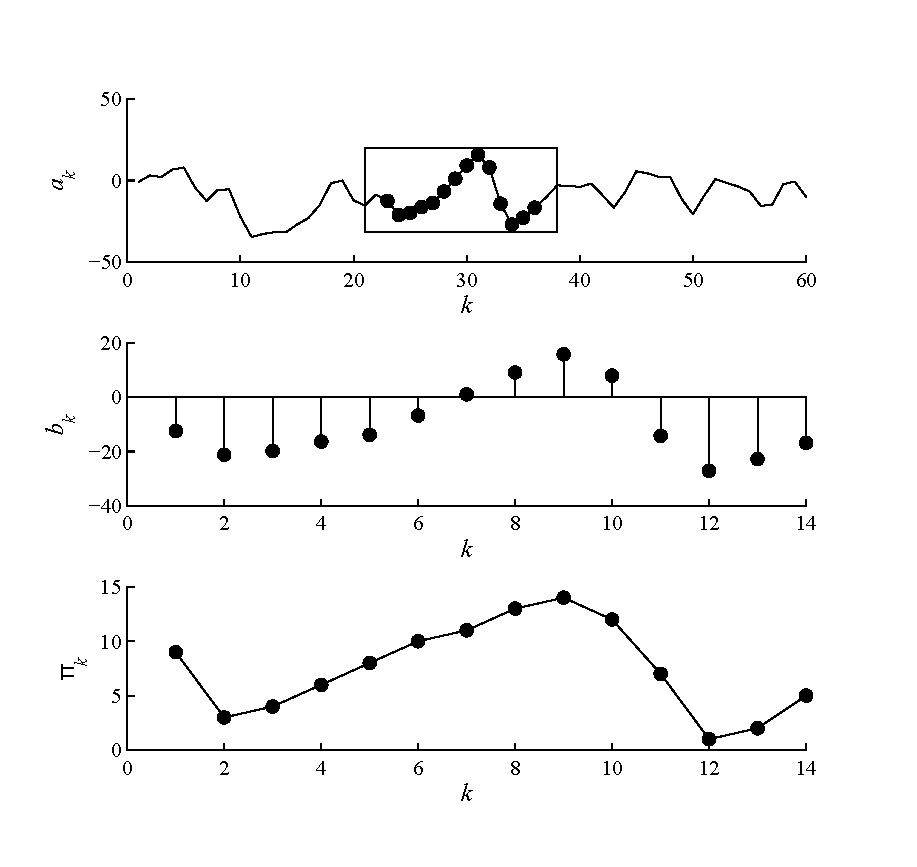
\includegraphics[width=10cm]{images/applicationToEEG.pdf}
	\caption{Permutation analysis of EEG: original EEG (top), windowed signal for $w=14$ (middle), permutation pattern(bottom)}
	\label{img:top}
\end{figure} 

\begin{figure}[h]
	\centering
   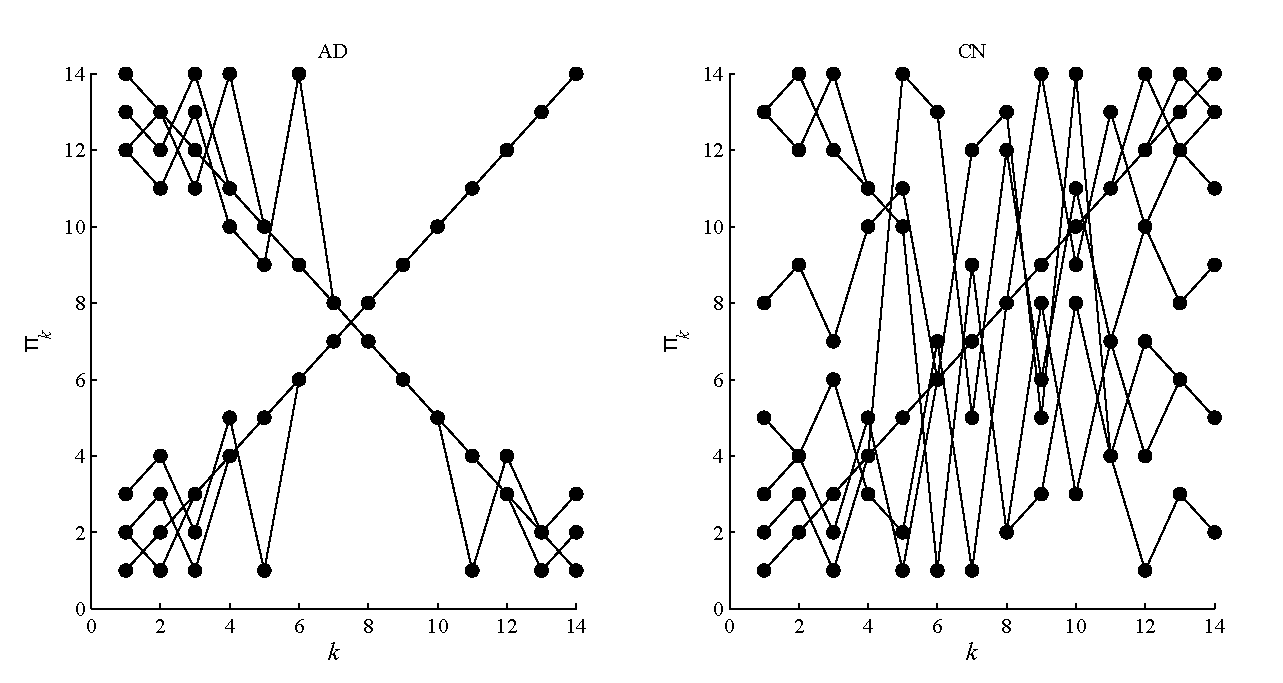
\includegraphics[width=13cm]{images/freqventPerm.pdf}
	\caption{Top 10 frequent permutations of two typical patients ($w$=14, $ch$=8)}
	\label{img:compare}
\end{figure}

\begin{figure}[h]
	\centering
   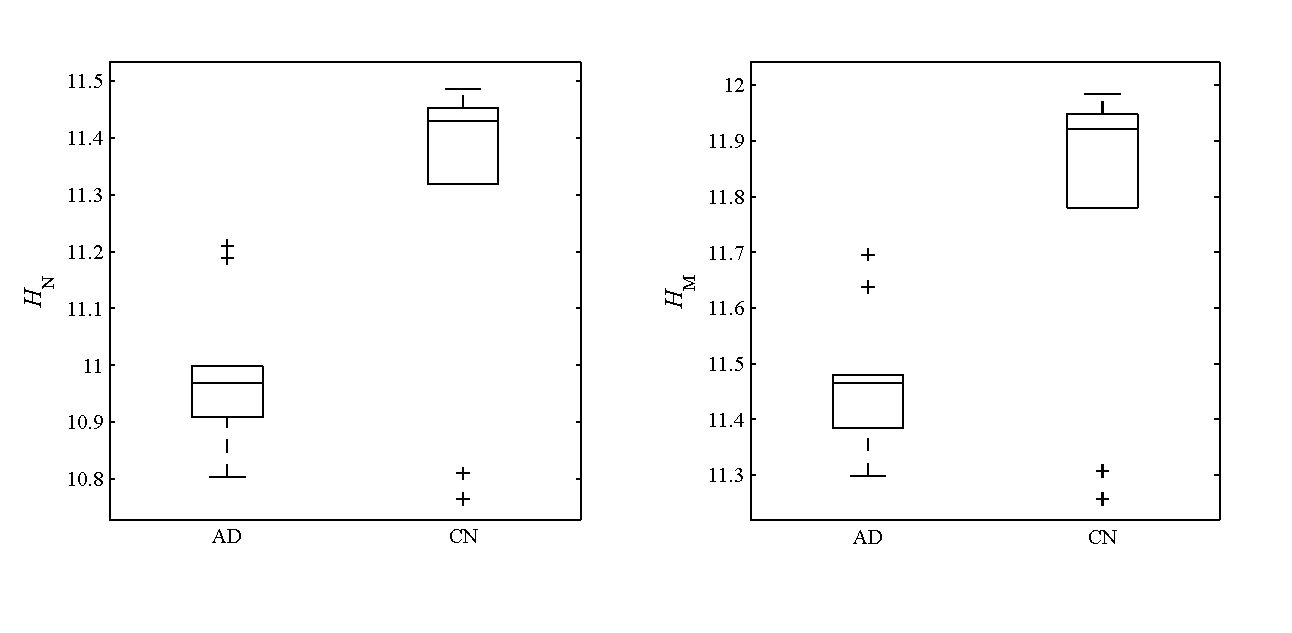
\includegraphics[width=13cm]{images/boxes.pdf}
	\caption{Permutation entropies for AD and CN ($w$=14, $ch$=8): naive (left) and Miller (right) approaches}
	\label{img:boxes}
\end{figure}

\newpage

\begin{appendices}
\section {Main function for permutation}
\ttfamily
\begin{lstlisting}
function [Hn, Hm] = PERMENTROPY(a, w)
    n = HASHPERM( a, w );
    [Hn, Hm] = ENTROPIES(n);
end
\end{lstlisting}

\normalfont
\section {Hash function}
\ttfamily
\begin{lstlisting}
function [n, PI] = HASHPERM(a, w)
    lena  = length(a);
    ns = lena - w + 1;
    nhash = 3*ns;
    nhash = nextprime(nhash);
    PI = zeros(nhash, w);
    n = zeros(nhash, 1);

    for k=1:ns
        [s, pi] = sort(a(k:k+w-1));
        index = 0;
        for j=1:w
            index = w*index+pi(j)-1;
            index = mod(index, nhash)+1;
        end 
        if n(index)==0
            n(index) = n(index) + 1;
            PI(index,:) = pi;
        else
            while n(index)>0
                if abs(PI(index,:)-pi) == 0
                    n(index) = n(index) + 1;
                    break
                end
                index = index + 1;
                if index > nhash
                    index = 1;
                end
                if n(index)==0
                    n(index) = n(index) + 1;
                    PI(index,:) = pi;
                    break
                end
            end
        end
    end

    n = n(n>0);
    n(end+1)=0;

    if nargout == 2
        PI(all(PI==0,2),:)=[];
    end
end
\end{lstlisting}

\normalfont
\section {Main function for entropy}
\ttfamily
\begin{lstlisting}
function [Hn, Hm] = ENTROPIES(n)
    L=length(n);
    N=sum(n);
    Hn=SHANNONENTROPY(n/N);
    Hm=SHANNONENTROPY(n/N)+(L-1)/2/N;
end
\end{lstlisting}

\normalfont
\section {Shannon entropy}
\ttfamily
\begin{lstlisting}
function [H] = SHANNONENTROPY(p)
    p=p(p>0);
    H=-sum(p.*log(p));
end
\end{lstlisting}

\end{appendices}

\end{document}
